\documentclass[11pt]{amsart}
\usepackage[a4paper,margin=1in]{geometry}
\usepackage{amssymb,tikz}
\usetikzlibrary{calc,arrows.meta}
\usepackage[hidelinks]{hyperref}
\hypersetup{pdftitle={Four Acute Faces: An Antipodal Counting Proof},pdfauthor={Vamshi Jandhyala}}
\newtheorem{theorem}{Theorem}
\newtheorem{lemma}[theorem]{Lemma}
\newcommand{\E}{\mathbb E}\newcommand{\R}{\mathbb R}
\newcommand{\shape}[1]{\begin{tikzpicture}[x=6pt,y=6pt,baseline=-4pt]
\foreach \n [count=\i] in {#1}{\foreach \j in {1,...,\n}{
\fill[black!20] (\j,-\i) rectangle +(1,-1);
\draw[line width=.5pt] (\j,-\i) rectangle +(1,-1);}}
\end{tikzpicture}}
\title[Four Acute Faces]{Four Acute Faces: An Antipodal Counting Proof}
\author{Vamshi Jandhyala}
\address{London, United Kingdom}
\email{vamshi.jandhyala@gmail.com}
\subjclass[2020]{60D05, 52A22}
\keywords{Geometric probability, random tetrahedron, antipodal symmetry}
\date{6 October 2026}
\begin{document}
\raggedbottom
\begin{abstract}
Four independent uniform points on the unit sphere form a tetrahedron
whose four faces are all acute with probability exactly $1/12$. We give a
self-contained exposition of the antipodal counting proof that first
appeared in a conversation publicly shared by Timothy Chow. Antipodal flips
turn the dependent angle conditions into a $4\times4$ table of vector sums
whose marked entries form one of six corner shapes. Our contribution is the
organisation: one table for all twelve angle tests, a counting identity
expressed through the faces of a single tetrahedron, and a shorter final
calculation using one spherical cap.
\end{abstract}
\maketitle
\enlargethispage{3pt}

\section{Antipodal flips}
Choose four points independently and uniformly on the unit sphere in $\R^3$.
What is the probability that their tetrahedron has four acute faces? A single
face is acute with probability $1/2$~\cite[Lemma 4]{AEN}, but the faces are
dependent, so multiplying four such probabilities does not give the answer.

Before trying to average twelve angle conditions, consider
\begin{equation}\label{eq:example}
 a=\tfrac13(-2,-1,2),\quad b=(1,0,0),\quad
 c=\tfrac13(-2,1,2),\quad d=\tfrac13(-1,2,2).
\end{equation}
Consider the angle at $c$ in $acd$, before and after replacing $c$ by $-c$.
The first dot product is $(a-c)\cdot(d-c)=-2/9$. After the replacement,
the three angle dot products in $a(-c)d$ are $4/9$, $28/9$ and $2/3$.
The face has become acute. In fact $(a,-b,-c,d)$ has four acute faces;
the table below will verify all twelve angles at once. For these points,
exactly one of the eight tetrahedra up to overall reflection succeeds.

The question was posed on MathOverflow and Mathematics Stack
Exchange~\cite{MO,MSE}. On 14 August 2026, Timothy Chow linked a publicly
shared ChatGPT conversation containing two complete proofs of the value
$1/12$~\cite{ChowChat}. The result, the antipodal mechanism, the total-sum
threshold and the linear-dependence argument below are already in that
conversation. Our purpose is expository: organise the proof in one table and
express the count through the faces of one tetrahedron, simplifying the final
averaging calculation. The author posted a version of the argument on
MathOverflow on 1 October 2026~\cite{MOAnswer}, found with Claude (Anthropic)
but without having read that conversation.

Related exact computations in geometric probability include Wendel's
centre-containment probabilities~\cite{Wendel}, Hall's acute-triangle
probabilities for points in a ball~\cite{Hall}, and Kabluchko's expected
solid-angle sums of random inscribed simplices~\cite{Kab}.

The proof has three steps. First, antipodal flips turn the twelve angle
conditions into a placement rule for sixteen triple sums. Second, the sums
occupy a corner of a $4\times4$ table, and counting its six possible shapes
gives an identity relating successful tetrahedra to their short face sums.
Third, one spherical-cap calculation and one integral give the two expectations
needed to obtain $1/12$.

\section{The angle criterion}
The example suggests using antipodes: replacing any chosen point by its
negative preserves its uniform distribution. The $16$ choices of signs form
eight pairs under overall reflection, which preserves angles. We keep $a$
fixed and let $T_X$ denote the tetrahedron obtained by flipping the vertices
in $X\subseteq\{b,c,d\}$. Write $N$ for the number of these eight tetrahedra
having four acute faces. Its value is $1$ for our example; $\E N$ averages
this count over random choices of the four points. If $p$ is the desired
probability, symmetry and
linearity of expectation give
\begin{equation}\label{eq:EN}
 \E N=8p.
\end{equation}
The eight tetrahedra are dependent; this equality does not require their
independence.

In the failed face above, $\|a+d-c\|^2=5/9$ and
$-2/9=(5/9-1)/2$. The angle test has a particularly useful form
(Figure~\ref{fig:angle}).
\begin{lemma}\label{lem:angle}
For unit vectors $x,y,z$,
\[
 (x-z)\cdot(y-z)=\tfrac12\bigl(\|x+y-z\|^2-1\bigr).
\]
Thus the angle at $z$ in $xyz$ is obtuse precisely when $\|x+y-z\|<1$.
\end{lemma}
\begin{proof}
Both sides expand to $x\cdot y-x\cdot z-y\cdot z+1$.
\end{proof}

\begin{figure}[ht]
\centering
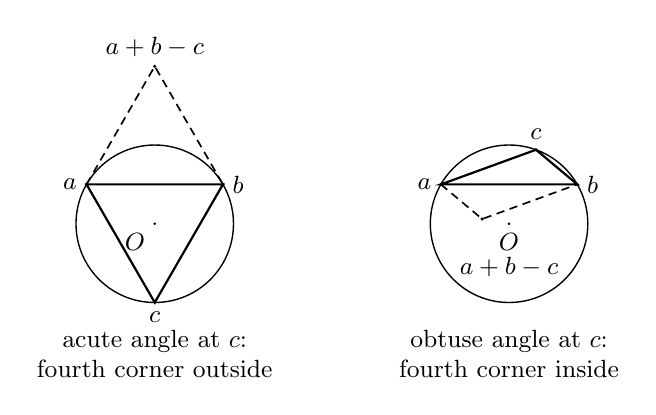
\begin{tikzpicture}% Drawn directly at publication size: no document-level scaling.
% Labels 9 pt, strokes at least 0.5 pt; total width below 5 inches.
\begin{scope}[every node/.style={font=\fontsize{9}{11}\selectfont}]
\coordinate (A) at (-.866,.5); \coordinate (B) at (.866,.5);
\coordinate (C) at (0,-1); \coordinate (D) at (0,2);
\draw[line width=.5pt] (0,0) circle (1);
\draw[densely dashed,line width=.6pt] (A)--(D)--(B);
\draw[line width=.8pt] (A)--(B)--(C)--cycle;
\fill (0,0) circle (.018) node[below left] {$O$};
\foreach \p/\l/\a in {A/a/left,B/b/right,C/c/below,D/{a+b-c}/above}
 {\fill (\p) circle (.022);\node[\a] at (\p) {$\l$};}
\node[align=center] at (0,-1.65) {acute angle at $c$:\\fourth corner outside};
\end{scope}
\begin{scope}[xshift=4.5cm,every node/.style={font=\fontsize{9}{11}\selectfont}]
\coordinate (A) at (-.866,.5); \coordinate (B) at (.866,.5);
\coordinate (C) at (.342,.940); \coordinate (D) at (-.342,.060);
\draw[line width=.5pt] (0,0) circle (1);
\draw[densely dashed,line width=.6pt] (A)--(D)--(B);
\draw[line width=.8pt] (A)--(B)--(C)--cycle;
\fill (0,0) circle (.018) node[below] {$O$};
\foreach \p/\l/\a in {A/a/left,B/b/right,C/c/above}
 {\fill (\p) circle (.022);\node[\a] at (\p) {$\l$};}
\fill (D) circle (.022);\node at (0,-.55) {$a+b-c$};
\node[align=center] at (0,-1.65) {obtuse angle at $c$:\\fourth corner inside};
\end{scope}
\end{tikzpicture}
\caption{The fourth corner $x+y-z$ of the parallelogram on the sides at $z$
lies outside the unit ball for an acute angle and inside for an obtuse one
(the diagram uses $a,b,c$ in place of $x,y,z$).}
\label{fig:angle}
\end{figure}

Our example has $\|a-c+d\|^2=5/9<1$. Call a vector sum
\emph{short} if its norm is less than $1$. Before the flip it tests the
obtuse angle at $c$; afterwards it is the vertex sum of $a(-c)d$ and tests
no angle of that face. This change of role is what we need to track.

On each triple of antipodal pairs, the four triangles up to reflection have
vertex sums
\[
 x+y+z,\qquad -x+y+z,\qquad x-y+z,\qquad x+y-z.
\]
Flipping two vertices is, up to reflection, equivalent to flipping the third.
There are four triples of pairs, hence sixteen labelled sums up to sign.
For any one tetrahedron, four of these entries are its face vertex sums and
the other twelve are its angle tests. Labels remain distinct even if vector
sums coincide. We disregard sums of norm exactly $1$, a null event justified
in Section~\ref{sec:caps}.

\begin{lemma}\label{lem:criterion}
A tetrahedron has four acute faces if and only if every short entry in the
sixteen-entry list is among its four face vertex sums.
\end{lemma}
\begin{proof}
By Lemma~\ref{lem:angle}, all twelve angles are acute exactly when all twelve
angle-test sums have norm greater than $1$. The only remaining entries are
the four face sums.
\end{proof}

\section{The table}
A triangle belongs to two tetrahedra, obtained by either choice of the fourth
vertex. For example, $a,-c,d$ belongs to $T_c$ and $T_{bc}$, which flip one
and two vertices respectively. Put the even choices
$T_\varnothing,T_{bc},T_{bd},T_{cd}$ in rows and the odd choices
$T_b,T_c,T_d,T_{bcd}$ in columns, placing a triangle in the cell of its two
containing tetrahedra.

To see why every cell holds exactly one triangle class, start with two
examples. The pair $T_\varnothing,T_b$ differs only at $b$, so its common
face is $a,c,d$. The pair $T_\varnothing,T_{bcd}$ appears to differ at three
vertices, but reflecting $T_{bcd}$ gives $(-a,b,c,d)$, revealing their common
face $b,c,d$.

In general, an even and an odd choice differ at one or three of $b,c,d$.
With one difference, the other three vertices give their unique common face.
With three differences, reflection turns the pair into tetrahedra differing
only at $a$, again giving a unique common face up to reflection.

Conversely, each triangle class belongs to one even and one odd tetrahedron.
Choosing the fourth vertex from a $b,c,d$ pair changes the parity by one flip.
If the missing pair is $a$, reflecting to keep $a$ fixed complements all
three other signs, also switching even and odd. Thus every triangle class
occupies exactly one cell, and all sixteen cells are filled.

Mark a cell if its vertex sum is short. A tetrahedron's line contains its
four face sums; the twelve cells outside it are its angle tests. Thus
Lemma~\ref{lem:criterion} says that a tetrahedron succeeds exactly when its
line contains every mark. The example in Table~\ref{tab:main} has two marks
in row $T_{bc}$ and therefore $N=1$.

The cell of $T_{bc}$ and $T_c$ has squared tetrahedron totals $20/9$ and
$8/9$, adding to $28/9<4$; its face sum has squared norm $5/9<1$.
The table also determines which cells are marked without testing each vector
separately. Let $x_i$ and $y_j$ be the squared norms of the four-vertex totals
of row $i$ and column $j$. If their common face has vertex sum $L$ and the
remaining pair is $\pm A$, their totals are $L+A$ and $L-A$, up to sign.
The parallelogram law gives
\begin{equation}\label{eq:threshold}
 x_i+y_j=\|L+A\|^2+\|L-A\|^2=2\|L\|^2+2.
\end{equation}
Consequently a cell is marked exactly when $x_i+y_j<4$. Sorting rows and
columns by increasing squared totals makes the marks an upper-left corner:
a marked cell forces every cell above it and to its left to be marked.

\begin{table}[ht]
\caption{One table for~\eqref{eq:example}: entries are common-face vertex
sums, up to sign; the margins give squared tetrahedron totals. A cell is
marked when its two margins add to less than $4$. The two marked entries
(bold) have squared norm $5/9$. Row $T_{bc}$ contains both; each of its twelve
off-row entries is an acute-angle test.}
\centering\small\setlength{\tabcolsep}{2.5pt}\renewcommand{\arraystretch}{1.2}
\begin{tabular}{c r|cccc}
 & & $T_d$ & $T_c$ & $T_{bcd}$ & $T_b$\\
 & $x_i\backslash y_j$ & $8/9$ & $8/9$ & $24/9$ & $104/9$\\\hline
$T_{bc}$ & $20/9$ & $\boldsymbol{-b-c+d}$ & $\boldsymbol{a-c+d}$ & $a-b-c$ & $a-b+d$\\
$T_{cd}$ & $36/9$ & $a+b-d$ & $a+b-c$ & $a-c-d$ & $b-c-d$\\
$T_\varnothing$ & $44/9$ & $a+b+c$ & $a+b+d$ & $b+c+d$ & $a+c+d$\\
$T_{bd}$ & $44/9$ & $a+c-d$ & $-b+c-d$ & $a-b-d$ & $a-b+c$
\end{tabular}
\label{tab:main}
\end{table}

\section{Restrictions on the marks}
We now show that the marked corner is nonempty, has at most three marks in
any line and has at most four marks in all. Averaging the four face sums
gives the first two facts, and the parallelogram law gives the third. The nonemptiness argument is where
dimension $3$ enters.

For the example's $T_{bc}$, the four squared face sums are $5/9$, $5/9$,
$53/9$ and $13/9$. Their average is $19/9>1$. The tetrahedron's total is
$S=(-4,0,2)/3$, so this is $1+\|S\|^2/2$. An average above $1$ cannot
force a short sum. To force one, we look for nonnegative weights totalling
$1$ that make the weighted average exactly $1$; the following identity
shows how to choose them.

For unit vertices $B_1,\ldots,B_4$ and total $S=\sum_iB_i$, the face sums
are $S-B_i$. If $\beta_i\ge0$ and $\sum_i\beta_i=1$, then
\begin{equation}\label{eq:average}
 \sum_i\beta_i\|S-B_i\|^2
 =\|S\|^2+1-2S\cdot\sum_i\beta_iB_i.
\end{equation}
The left side averages squared face sums; the right side shows that making
the weighted vertex sum $S/2$ will make that average $1$.

\begin{lemma}\label{lem:restrictions}
The marked corner is nonempty, has at most three marks in any line, and has
at most four marks in total.
\end{lemma}
\begin{proof}
Equal weights $\beta_i=1/4$ in~\eqref{eq:average} give
$1+\|S\|^2/2\ge1$. Thus the four face sums cannot all be short, excluding
a line of four marks.

For nonemptiness, half-weights give vertex sum $S/2$ but total weight $2$.
We must subtract weights totalling $1$ whose vertex sum is zero. In the
example, $3a-2b-9c+6d=0$ becomes a positive relation for $T_{bc}$;
normalising gives $w=(3,2,9,6)/20$. Subtract these from the half-weights:
\[
\begin{array}{r|rrrr|c|c}
 &a&-b&-c&d&\text{weight total}&\text{vertex sum}\\
\tfrac12\text{ each}&10/20&10/20&10/20&10/20&2&S/2\\
\text{minus }w&3/20&2/20&9/20&6/20&1&0\\\hline
\beta&7/20&8/20&1/20&4/20&1&S/2
\end{array}
\]
This subtraction corrects the total weight without changing the vertex sum,
so~\eqref{eq:average} makes the squared-face average exactly $1$. Indeed,
with the squared face sums $5/9,5/9,53/9,13/9$ opposite $a,-b,-c,d$,
\[
 \frac{7\cdot5+8\cdot5+1\cdot53+4\cdot13}{20\cdot9}=1.
\]

In general, four vectors in $\R^3$ have a nonzero linear relation. Flip
vertices with negative coefficients; zero coefficients stay zero. Normalising
the now nonnegative, not-all-zero coefficients produces one of the eight
tetrahedra and weights $w_i\ge0$ with $\sum_iw_i=1$ and
$\sum_iw_iB_i=0$. Each satisfies
\[
 w_i=\Big\|\sum_{j\ne i}w_jB_j\Big\|\le\sum_{j\ne i}w_j=1-w_i.
\]
Thus $\beta_i=1/2-w_i$ are nonnegative, sum to $1$ and have vertex sum
$S/2$. Equation~\eqref{eq:average} gives average $1$, so some face sum has
norm at most $1$, hence less than $1$ under our null-set convention.

Finally, two distinct triangle classes on the same triple of pairs differ,
after reflection if needed, by one flip. Their sums are $u+v$ and $u-v$ with
$\|v\|=1$, so their squared norms add to $2\|u\|^2+2\ge2$.
They cannot both be short. There are four triples of pairs, giving at most
four marks altogether.
\end{proof}

\section{The counting identity}
In Table~\ref{tab:main}, $T_{bc}$ has two short face sums, $T_c$ and $T_d$
have one each, and the other five tetrahedra have none. Let $k$ count the
short face sums of one tetrahedron and let $C$ count the tetrahedra with
$k=1$ or $2$. The example has $C=3$ and $N=1$. The facts of
Lemma~\ref{lem:restrictions} matter here: an empty table would give
$N+C=8$, and a fully marked row would give $N=1$ and $C=4$.

\begin{lemma}\label{lem:count}
For every configuration outside the excluded null set, $N+C=4$.
\end{lemma}
\begin{proof}
By Lemma~\ref{lem:restrictions}, the corner contains between one and four
marks, with at most three per line. List its nonzero row lengths. Up to
transposition, which changes neither count, there are six possibilities:
\[
\begin{array}{c|c|c|c|c}
\text{shape}&\text{row lengths}&\text{column lengths}&N&C\\\hline
\shape{1}&1&1&2&2\\
\shape{2}&2&1,1&1&3\\
\shape{3}&3&1,1,1&1&3\\
\shape{2,1}&2,1&2,1&0&4\\
\shape{3,1}&3,1&2,1,1&0&4\\
\shape{2,2}&2,2&2,2&0&4
\end{array}
\]
Here $N$ counts lines containing every mark, while $C$ counts lines with
one or two marks. For instance, in shape $(2,1)$ no line contains every mark,
but the two nonempty rows and two nonempty columns each count towards $C$.
Every row of the displayed list gives $N+C=4$.
\end{proof}

Taking expectations, using~\eqref{eq:EN} and the equal distributions of
the eight tetrahedra, gives
\[
 p=\tfrac12-\Pr(k=1\text{ or }2).
\]
Two short faces give one pair, and three give three pairs. Writing the pair
count as $\binom k2$, and recalling $k\le3$, these counts encode precisely
this event:
\[
\begin{array}{c|rrrr}
k&0&1&2&3\\
\binom k2&0&0&1&3\\
k-\binom k2&0&1&1&0.
\end{array}
\]
In words, the number of short face sums minus their number of pairs is
the indicator of $k=1$ or $2$. Therefore
\begin{equation}\label{eq:moments}
 p=\tfrac12+\E\binom k2-\E k.
\end{equation}
We now need only the probability of one short sum and of a pair sharing two
vertices.

\section{The cap calculation}\label{sec:caps}
The cap below height $-1/2$ occupies $1/4$ of the unit sphere. More generally,
Archimedes' hat-box theorem makes a uniform point's height along any fixed
axis uniform on $[-1,1]$: a band of height $h$ has area $2\pi h$.
\footnote{At height $z$, the ring radius is $r=\sqrt{1-z^2}$. The circumference
$2\pi r$ times the sloping width per unit height
$\sqrt{1+(dr/dz)^2}=1/r$ gives constant area density $2\pi$.
Integrating gives the band area, with pole endpoints understood by limits.}

Fix $a,b$, and write $s=\|a+b\|$. Since
\[
 \|a+b+c\|^2=s^2+1+2c\cdot(a+b),
\]
the sum is short when the height of $c$ along $(a+b)/s$ is below $-s/2$.
Thus the cap has height $1-s/2$ and probability
\begin{equation}\label{eq:q}
 q=\frac{2-s}{4}.
\end{equation}
For example, $a\cdot b=-1/2$ gives $s=1$ and $q=1/4$; independent $c,d$
both hit that fixed cap with probability $1/16$.
Norm-one equality cases have probability zero: for $s>0$,
the squared norm above is uniform on an interval of positive length, and
$s=0$ itself has probability zero. Sign symmetry applies this argument to
each of the sixteen labelled sums, justifying the earlier exclusion.

\begin{figure}[ht]
\centering
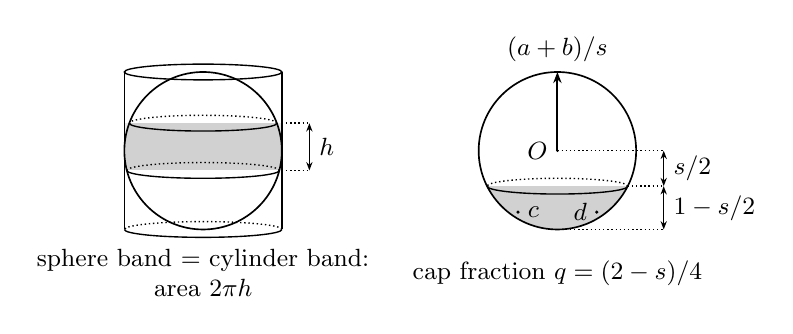
\begin{tikzpicture}% Drawn directly at publication size, with 9 pt labels and >= 0.5 pt strokes.
\begin{scope}[every node/.style={font=\fontsize{9}{11}\selectfont}]
\fill[black!8] (-1,-.25) rectangle (1,.35);
\draw[line width=.5pt] (-1,-1)--(-1,1) (1,-1)--(1,1);
\draw[line width=.5pt] (0,1) ellipse (1cm and .1cm);
\draw[line width=.5pt] (1,-1) arc (0:-180:1cm and .1cm);
\draw[line width=.5pt,densely dotted] (1,-1) arc (0:180:1cm and .1cm);
\begin{scope}\clip (0,0) circle (1);\fill[black!18] (-1.1,-.25) rectangle (1.1,.35);\end{scope}
\draw[line width=.6pt] (0,0) circle (1);
\foreach \z in {-.25,.35} {
 \pgfmathsetmacro{\r}{sqrt(1-\z*\z)}
 \draw[line width=.5pt] (\r,\z) arc (0:-180:\r cm and .1cm);
 \draw[line width=.5pt,densely dotted] (\r,\z) arc (0:180:\r cm and .1cm);
}
\draw[line width=.5pt,{Stealth[length=3pt]}-{Stealth[length=3pt]}] (1.35,-.25)--node[right] {$h$}(1.35,.35);
\draw[line width=.5pt,densely dotted] (1,-.25)--(1.35,-.25) (1,.35)--(1.35,.35);
\node[align=center] at (0,-1.55) {sphere band = cylinder band:\\area $2\pi h$};
\end{scope}
\begin{scope}[xshift=4.5cm,every node/.style={font=\fontsize{9}{11}\selectfont}]
\begin{scope}\clip (0,0) circle (1);\fill[black!18] (-1.1,-1.1) rectangle (1.1,-.45);\end{scope}
\draw[line width=.6pt] (0,0) circle (1);
\pgfmathsetmacro{\r}{sqrt(1-.45*.45)}
\draw[line width=.5pt] (\r,-.45) arc (0:-180:\r cm and .1cm);
\draw[line width=.5pt,densely dotted] (\r,-.45) arc (0:180:\r cm and .1cm);
\fill (0,0) circle (.018) node[left] {$O$};
\draw[line width=.7pt,-{Stealth[length=4pt]}] (0,0)--(0,1) node[above] {$(a+b)/s$};
\draw[line width=.5pt,{Stealth[length=3pt]}-{Stealth[length=3pt]}] (1.35,0)--node[right] {$s/2$}(1.35,-.45);
\draw[line width=.5pt,{Stealth[length=3pt]}-{Stealth[length=3pt]}] (1.35,-.45)--node[right] {$1-s/2$}(1.35,-1);
\draw[line width=.5pt,densely dotted] (0,0)--(1.35,0) (\r,-.45)--(1.35,-.45) (0,-1)--(1.35,-1);
\fill (-.5,-.78) circle (.022) node[right] {$c$};
\fill (.5,-.78) circle (.022) node[left] {$d$};
\node at (0,-1.55) {cap fraction $q=(2-s)/4$};
\end{scope}
\end{tikzpicture}
\caption{Equal-height sphere and cylinder bands have equal area (left).
Both face sums $a+b+c$ and $a+b+d$ are short when $c,d$ hit the same cap of
height $1-s/2$ (right).}
\label{fig:cap}
\end{figure}

Let $\alpha=\E q$ be the probability that one face sum is short. Two face
sums share two vertices, so their probability of both being short is
$\gamma=\E(q^2)$: fix $a,b$, multiply the two independent cap probabilities,
then average. The shared random cap is why squaring must precede averaging.
Four faces and six pairs give $\E k=4\alpha$ and
$\E\binom k2=6\gamma$.

It is useful to average the hit--miss probability $q(1-q)$, whose factors
remove the square root in $s$:
\[
 q(1-q)=\frac{(2-s)(2+s)}{16}=\frac{4-s^2}{16},
 \qquad \E s^2=2+2\E(a\cdot b)=2.
\]
The last mean vanishes by the symmetry $b\leftrightarrow-b$. Hence
$\alpha-\gamma=1/8$, and~\eqref{eq:moments} reduces to
\[
 p=\tfrac12+6\gamma-4\alpha=2\alpha-\tfrac14.
\]
Finally, $U=(1+a\cdot b)/2$ is uniform on $[0,1]$ and $s=2\sqrt U$, so
\[
 \alpha=\int_0^1\frac{1-\sqrt u}{2}\,du=\frac16,
 \qquad p=2\cdot\frac16-\frac14=\boxed{\frac1{12}}.
\]
As a check, $\alpha$ is also the probability that a specified angle of an
inscribed random triangle is obtuse. Its three angles have equal distributions
and at most one is obtuse, giving acute-triangle probability $1-3\alpha=1/2$.

\section{Remarks}
The varying success count $N\in\{0,1,2\}$ is what prevents a constant-flip
argument of the kind used for centre containment~\cite{Wendel}.
The earlier proof~\cite{ChowChat} counts $N=4-2m+J$, where $m$ is the number
of short entries and $J$ counts pairs on a common line. Each entry lies on
two lines and two distinct entries share at most one line, so
$\sum_t k_t=2m$, $\sum_t\binom{k_t}{2}=J$ and $C=2m-J$.
Thus $N+C=4$ is the same identity expressed through the short face sums of
one tetrahedron; its advantage is the immediate reduction to two moments.

Dimension $3$ enters in the nonzero linear relation among four vertices.
For four orthonormal vectors in $\R^4$, every triple sum has squared norm
$3$: the table is empty and all eight tetrahedra have equilateral faces.
The short-sum angle test is unchanged, but the nonemptiness argument fails.

\section*{Acknowledgements}
This paper was developed with Claude (Anthropic).
The author is responsible for the mathematics and citations. A portable
exact-arithmetic checker accompanies the source; its finite checks support,
but do not replace, the proof.

\begin{thebibliography}{9}
\bibitem{AEN} A.~Akopyan, H.~Edelsbrunner and A.~Nikitenko, \emph{The beauty of random polytopes inscribed in the $2$-sphere}, Experiment.\ Math.\ \textbf{34} (2025), no.~3, 327--341. \href{https://doi.org/10.1080/10586458.2021.1980459}{doi:10.1080/10586458.2021.1980459}.
\bibitem{ChowChat} \emph{Tetrahedron Acute Faces Proof}, ChatGPT-generated responses in a conversation publicly shared by Timothy Chow and linked in a MathOverflow comment on 14 August 2026. \url{https://chatgpt.com/share/6a7e8742-01e0-83ea-81de-533ea9dcb597}. Accessed 6 October 2026.
\bibitem{Hall} G.~R.~Hall, \emph{Acute triangles in the $n$-ball}, J.\ Appl.\ Probab.\ \textbf{19} (1982), no.~3, 712--715. \href{https://doi.org/10.2307/3213533}{doi:10.2307/3213533}.
\bibitem{Kab} Z.~Kabluchko, \emph{Angle sums of random simplices in dimensions $3$ and $4$}, Proc.\ Amer.\ Math.\ Soc.\ \textbf{148} (2020), no.~7, 3079--3086. \href{https://doi.org/10.1090/proc/14934}{doi:10.1090/proc/14934}.
\bibitem{MO} Dan, \emph{A tetrahedron's vertices are random points on a sphere. What is the probability that the tetrahedron's four faces are all acute triangles?}, MathOverflow question 498296 (2025), with answers and comments, \url{https://mathoverflow.net/q/498296}.
\bibitem{MSE} Dan, the same question on Mathematics Stack Exchange, question 5083355 (July 2025), with answers by J.~D'Aurizio and J.~Ferry, \url{https://math.stackexchange.com/q/5083355}.
\bibitem{MOAnswer} V.~Jandhyala, answer to MathOverflow question 498296, 1 October 2026, \url{https://mathoverflow.net/a/515661}.
\bibitem{Wendel} J.~G.~Wendel, \emph{A problem in geometric probability}, Math.\ Scand.\ \textbf{11} (1962), 109--111. \href{https://doi.org/10.7146/math.scand.a-10655}{doi:10.7146/math.scand.a-10655}.
\end{thebibliography}
\end{document}
